%%%%%%%%%%%%%%%%%%%%%%%%%%%%%%%%%%%%%%%%%
% Beamer Presentation
% LaTeX Template
% Version 1.0 (10/11/12)
%
% This template has been downloaded from:
% http://www.LaTeXTemplates.com
%
% License:
% CC BY-NC-SA 3.0 (http://creativecommons.org/licenses/by-nc-sa/3.0/)
%
%%%%%%%%%%%%%%%%%%%%%%%%%%%%%%%%%%%%%%%%%

%----------------------------------------------------------------------------------------
%	PACKAGES AND THEMES
%---------------------------------------------------------------------------------------- 
 
\documentclass[c]{beamer}
%\documentclass[notes]{beamer}
\setbeamertemplate{note page}[show only notes]
\input{OR_common.tex}
%%%%%%%%%%%%%%%%%%%%%%%%%%%%%%%%%%%%%%%%%%%%%%%%%%%%%%%%%%%%%%%%%%%%%%%%%%%%%
%%%%%%%%%%%%%%%%%%%%%%%%%%%%%%%%%%%%%%%%%%%%%%%%%%%%%%%%%%%%%%%%%%%%%%%%%%%%%
%%%%%%%%%%%%%%%%%%%%%%%%%%%%%%%%%%%%%%%%%%%%%%%%%%%%%%%%%%%%%%%%%%%%%%%%%%%%%

\title[Introduction]{Unit 3. Linear programming}

\author{Jordi Villà i Freixa}
\institute[FCTE]{
Universitat de Vic - Universitat Central de Catalunya \\
Study Abroad. Operations Research\\
\medskip
\textit{jordi.villa@uvic.cat\\\url{https://mon.uvic.cat/cbbl}}
}
\date{October 15th-29th, 2025\\last updated: \today}
\logo{
\includegraphics[width=.1\textwidth]{FCTE}}
\begin{document}

\begin{frame}
\titlepage
\end{frame}


\begin{frame}
    \frametitle{Preliminary}
    This course is strongly based on the monography on Operations Research by Carter, Price and Rabadi \cite{carter}, and in material obtained from different sources (quoted when needed through the slides).
\end{frame}

%%%%%%%%%%%%%%%%%%%%%%%%%%%%%%%%%%%%%%%%%%%%%%%%%%%%%%%%%%%%%%%%%%%%%%%%%%%%%
%%%%%%%%%%%%%%%%%%%%%%%%%%%%%%%%%%%%%%%%%%%%%%%%%%%%%%%%%%%%%%%%%%%%%%%%%%%%%
%%%%%%%%%%%%%%%%%%%%%%%%%%%%%%%%%%%%%%%%%%%%%%%%%%%%%%%%%%%%%%%%%%%%%%%%%%%%%

\section{Introduction to linear programming}

\begin{frame}
\frametitle{Learning outcomes}
\begin{itemize}
  \item Learn how to formulate a linear programming model
  \item Get familiar with the terms feasible region, feasible solutions and optimal feasible solutions
  \item Managing graphical solution of the linear programming model
  \item Identify models with unique, multiple or no optimal feasible solutions
  \item Introducing the Simplex method
\end{itemize}
\end{frame}


\begin{frame}{The linear programming model}

  \begin{block}{Linear programming}
    Linear programs consist of a linear objective function and linear constraints, which can include both equalities and inequalities. The feasible region forms a polytope —a convex, connected set with flat, polygonal faces. The contours of the objective function are flat planes.
   \cite{nocedal}
  \end{block}
  A wide variety of applications can be modeled with linear programming.

\end{frame}

\begin{frame}{Variables, function and bounds}
  Steps:
\begin{enumerate}
  \item identify the controllable decision variables $x_i$, with $i=1,\ldots,n$.
  \item establish the objective criterion: to either maximize or minimize some function of the form:
  \[
    z = c_1 x_1 +\cdots + c_n x_n = \sum_{i=1}^n c_i x_i
  \]
  where $c_i$ represents problem dependent constants.
  \item resource limitations and bounds on decision variables as linear equations or inequalities like
  \[
     a_1 x_1 +\cdots + a_n x_n \leq b
  \]
\end{enumerate}
\end{frame}

\begin{frame}{Linearization of problems}
  \begin{center}
    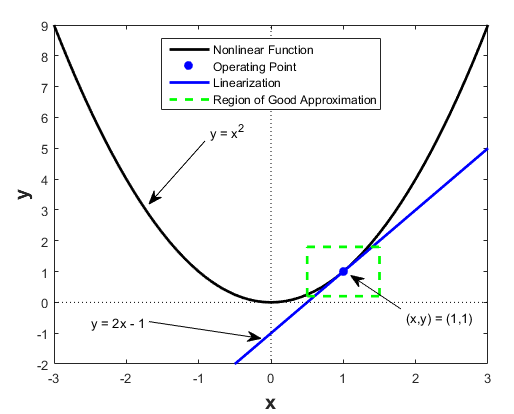
\includegraphics[width=0.45\linewidth]{linearization}
    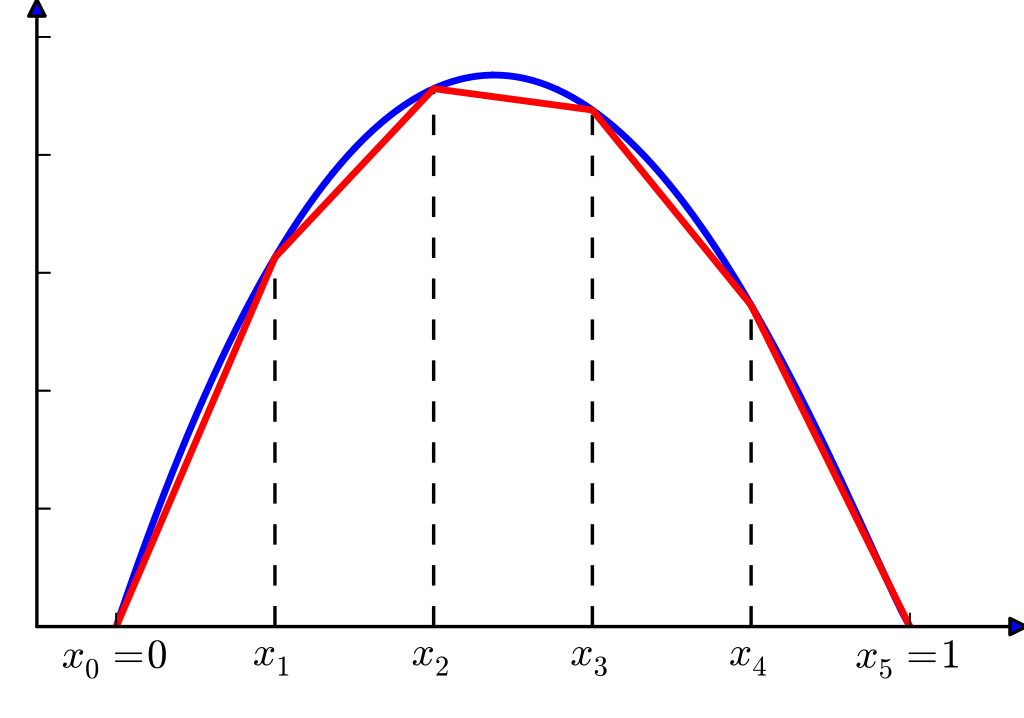
\includegraphics[width=0.45\linewidth]{PWLapprox}

  \href{https://es.mathworks.com/help/slcontrol/ug/linearizing-nonlinear-models.html}{Matlab example}
  \end{center}
\[
f(x) = f(a) + f'(a)(x - a) + \frac{f''(a)}{2!}(x - a)^2 + \cdots = \sum_{n=0}^{\infty} \frac{f^{(n)}(a)}{n!}(x - a)^n
\]

Linearization of \( f(x) = x^2 \) around \( x = 1 \): $f(x) \approx 1 + 2(x - 1) $
\end{frame}

\begin{frame}[allowframebreaks]{Problem formulation}
  \begin{Exercise}
    A manufacturer of computer system components assembles two models of wireless routers, model A and model B. The amounts of materials and labor required for each assembly, and the total amounts available, are shown in the following table. The profits that can be realized from the sale of each router are \$22 and \$28 for models A and B, respectively, and we assume there is a market for as many routers as can be manufactured.\cite{carter}
    \begin{center}
    \begin{tabular}{cccc}
      & Resources  & Resources  B & Resources  \\
      & per Unit A &  per Unit B &  available \\\hline
      Materials & 8 & 10 & 3400\\
      Labor & 2 & 3 & 960\\\hline
    \end{tabular}
  \end{center}
  How to maximize the benefits?
  \end{Exercise}
  \framebreak
  \begin{equation*}
    \begin{aligned}
      \text{maximize } \quad & z = 22 x_A+28x_B \\
      \text{subject to }\quad &
      \begin{array}{rcl}
        8x_A+10x_B &\leq &3400 \\
        2x_A+3x_B &\leq &960 \\
        x_A &\geq &0 \\
        x_B &\geq& 0
      \end{array}
    \end{aligned}
  \end{equation*}

\framebreak

  \begin{Exercise}
  A company wishes to minimize its combined costs of production and inventory over a four-week time period. An item produced in a given week is available for consumption during that week, or it may be kept in inventory for use in later weeks. Initial inventory at the beginning of week 1 is 250 units. The minimum allowed inventory carried from one week to the next is 50 units. Unit production cost is \$15, and the cost of storing a unit from one week to the next is \$3. The following table shows production capacities and the demands that must be met during each week.\cite{carter}
    \begin{center}
    \begin{tabular}{ccc}
      Period  & Production capacity & Demand  \\\hline
      1 &  800 &  900 \\
      2 & 700 & 600\\
      3 & 600 & 800\\
      4 & 800 & 600
    \end{tabular}
  \end{center}
  A minimum production of 500 items per week must be maintained. Inventory costs are not applied to items remaining at the end of the fourth production period, nor is the minimum inventory restriction applied after this final period.
  \end{Exercise}
  \framebreak
  Let $x_i$ be the number of units produced during the $i^{th}$ week, for $i = 1, …, 4$. The formulation is somewhat more manageable if we let $A_i$ denote the number of items remaining at the end of each week (accounting for those held over from previous weeks, those produced during the current week, and those consumed during the current week). Note that the $A_i$ values are not decision variables, but merely serve to simplify our written formulation. Thus,
  \begin{eqnarray*}
    A_1&=&250+x_1-900\\
    A_2&=&A_1+x_2-600\\
    A_3&=&A_2+x_3-800\\
    A_4&=&A_3+x_4-600
  \end{eqnarray*}
  \begin{equation*}
    \begin{aligned}
      \text{minimize } \quad & z = 15\cdot(x_1+x_2+x_3+x_4)+3\cdot (A_1+A_2+A_3) \\
      \text{subject to }\quad &
      \begin{array}{c}
        500 \leq x_1 \leq 700\\
        500 \leq x_2 \leq 700\\
        500 \leq x_3 \leq 600\\
        500 \leq x_4 \leq 800\\
        x_i \geq 0, \, i=1,2,3,4
      \end{array}
    \end{aligned}
  \end{equation*}
\end{frame}

\begin{frame}[c]{Integer problems}

  \begin{center}
    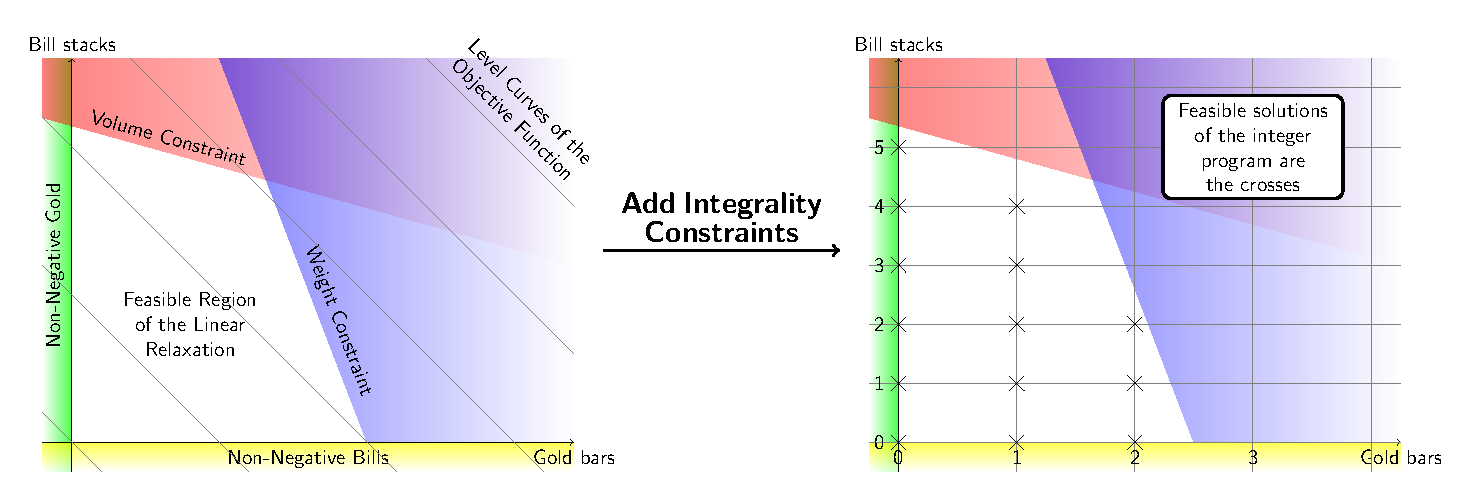
\includegraphics[width=\linewidth]{ILP.pdf}

    \href{http://www.science4all.org/article/integer-programming/}{from Lê Nguyên Hoang's http://www.science4all.org}
  \end{center}
\end{frame}

\subsection{Graphical solution}

\begin{frame}[c]{General issues}
  \begin{itemize}
    \item Remember: An optimal feasible solution is a point in the feasible space that is as effective as any other point in achieving the specified goal.
    \item The solution of linear programming problems with only two decision variables can be illustrated graphically.
    \item If an optimal feasible solution exists, it occurs at one of the extreme points of the feasible space.
    \item We illustrate this for problems with one, with multiple, and with none optimal feasible solutions.
  \end{itemize}
\end{frame}

\begin{frame}[allowframebreaks]{Unique optimal feasible solution}
  \begin{Exercise}
    \begin{equation*}
      \begin{aligned}
        \text{maximize } \quad & z = 3x_1 + x_2 \\
        \text{subject to }\quad &
        \begin{array}{rcl}
          x_2 & \leq & 5\\
          x_1 + x_2 &\leq& 10\\
          -x_1+x_2 &\geq& -2\\
          x_1,x_2 &\geq &0
        \end{array}
      \end{aligned}
    \end{equation*}
  \end{Exercise}
  \framebreak
  \begin{center}
    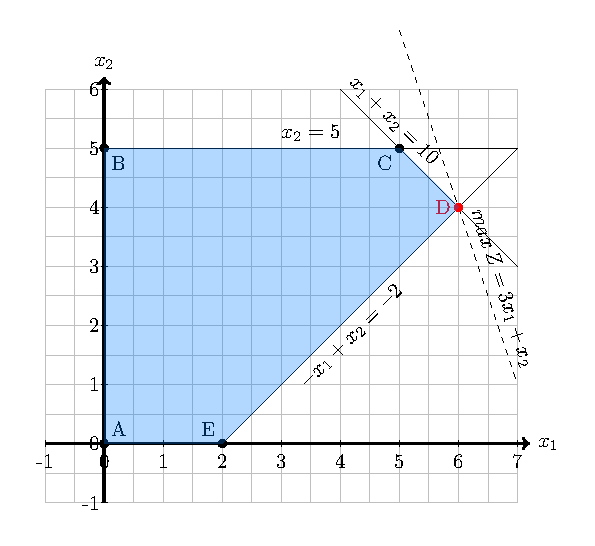
\includegraphics[width=0.6\linewidth]{LP2.pdf}
  \end{center}
 \framebreak
  \begin{Exercise}
    \begin{equation*}
      \begin{aligned}
        \text{minimize } \quad & z = x_1 + x_2 \\
        \text{subject to }\quad &
        \begin{array}{rcl}
          3x_1 + x_2 & \geq & 6\\
          x_2 &\geq& 3\\
          x_1 &\leq& 4\\
          x_1,x_2 &\geq &0
        \end{array}
      \end{aligned}
    \end{equation*}
  \end{Exercise}

 \framebreak
  \begin{center}
    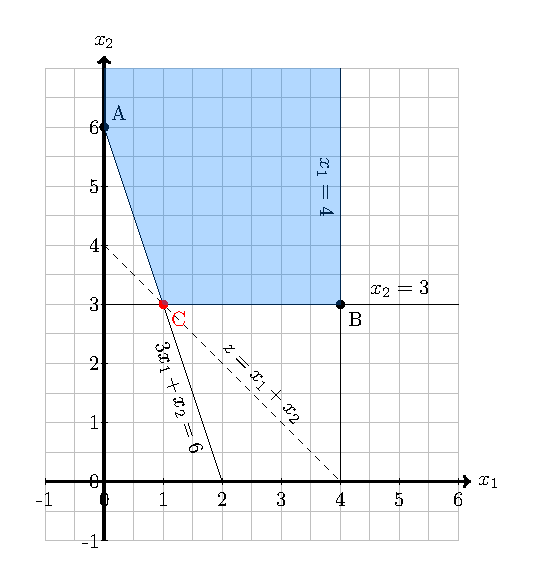
\includegraphics[width=0.6\linewidth]{LP6.pdf}
  \end{center}

\end{frame}

\begin{frame}[allowframebreaks]{Multiple optimal feasible solutions}
  \begin{Exercise}
    \begin{equation*}
      \begin{aligned}
        \text{maximize } \quad & z = x_1 + 2x_2 \\
        \text{subject to }\quad &
        \begin{array}{rcl}
          -x_1+x_2 & \leq & 2\\
          x_1 + 2x_2 &\leq& 8\\
          x_1 &\leq& 6\\
          x_1,x_2 &\geq &0
        \end{array}
      \end{aligned}
    \end{equation*}
  \end{Exercise}
 \framebreak
  %
  \begin{center}
   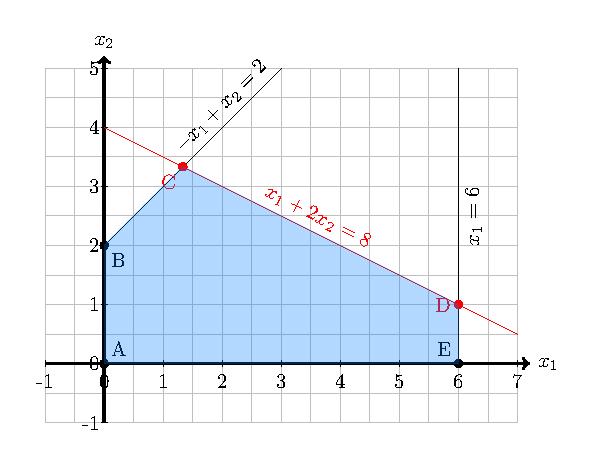
\includegraphics[width=0.7\linewidth]{LP3.pdf}
  \end{center}

\end{frame}

\begin{frame}[allowframebreaks]{No optimal feasible solutions}
  \begin{Exercise}
    \begin{equation*}
      \begin{aligned}
        \text{maximize } \quad & z = 3x_1 + x_2 \\
        \text{subject to }\quad &
        \begin{array}{rcl}
          x_1+x_2 & \geq & 4\\
          -x_1 + x_2 &\leq& 4\\
          -x_1 +2x_2 &\geq& -4\\
          x_1,x_2 &\geq &0
        \end{array}
      \end{aligned}
    \end{equation*}
  \end{Exercise}
  \framebreak
  \begin{center}
   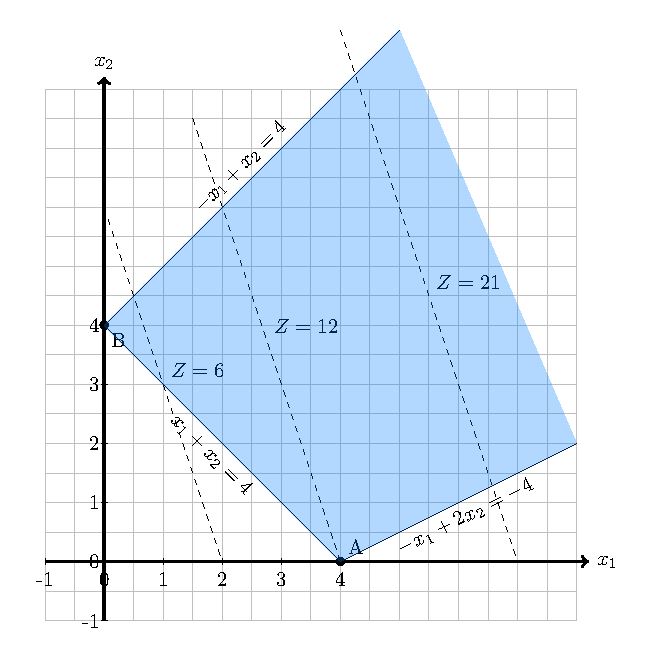
\includegraphics[width=0.7\linewidth]{LP4.pdf}
  \end{center}

\end{frame}

\begin{frame}[allowframebreaks]{No feasible solutions}
  \begin{Exercise}
    \begin{equation*}
      \begin{aligned}
        \text{maximize } \quad & z = 3x_1 + x_2 \\
        \text{subject to }\quad &
        \begin{array}{rcl}
          -x_1 + x_2 &\geq& 4\\
          -x_1 +2x_2 &\leq& -4\\
          x_1,x_2 &\geq &0
        \end{array}
      \end{aligned}
    \end{equation*}
  \end{Exercise}
  \framebreak
  \begin{center}
    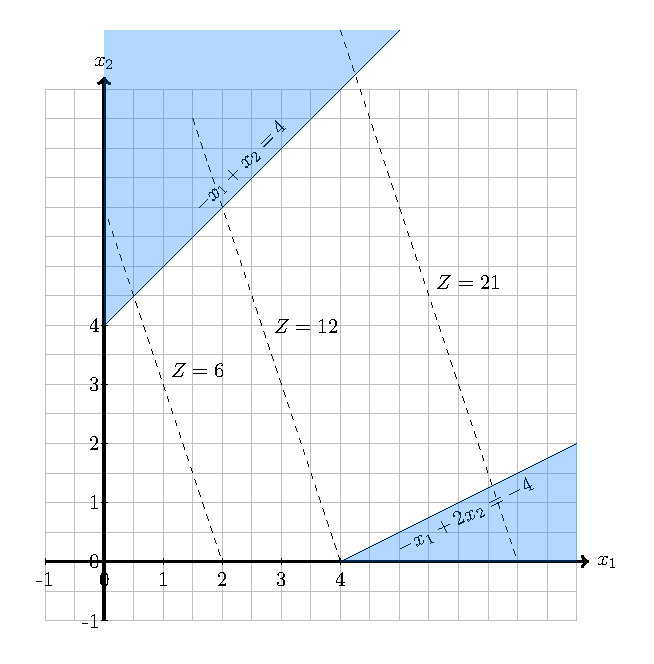
\includegraphics[width=0.7\linewidth]{LP5.pdf}
  \end{center}

\end{frame}

\subsection{General solution method}

\begin{frame}{General solution method of an LP problem}
  \begin{itemize}
    \item If an optimal solution exists, it occurs at an extreme point of the feasible region.
    \item Only the finitely many extreme points need be examined (rather than all the points in the feasible region).
    \item Thus, an optimal solution may be found systematically by considering the objective function values at the extreme points.
    \item In fact, in actual practice, only a small subset of the extreme points need be examined.
  \end{itemize}
  This is the foundation for a {\bf general solution method} of a LP problem called the {\bf Simplex method}.
\end{frame}

\section{Introduction to the Simplex method for LP}


\begin{frame}
\frametitle{Learning outcomes}
\begin{itemize}
  \item Understanding the rational behind the Simplex method for LP.
  \item Understanding and practicing the algorithm in 2 variables.
  \item Recognizing the different types of results one can achieve in LP from the Simplex Method algorithm.
  \item Getting familiar with slack, surplus and artificial variables.
\end{itemize}
\end{frame}


\begin{frame}
  \begin{center}
    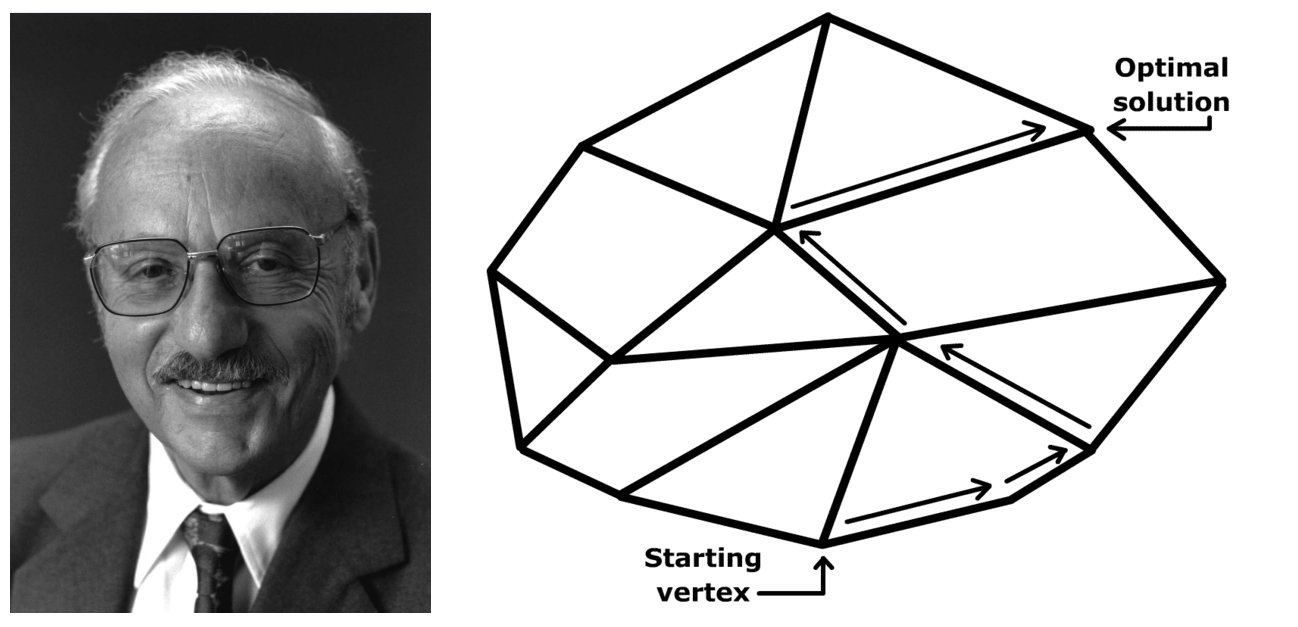
\includegraphics[width=\linewidth]{george-danzig-simplex.jpg}
  \end{center}

  Left: George Dantzig (1914-2005), the American mathematical scientist who devised linear programming and the simplex algorithm. Right: The simplex algorithm moves along the edges of the polytope until it reaches the optimum solution [Image Wikimedia Commons].
\end{frame}

\subsection{Preparing the LP problem for applying the Simplex method}

\begin{frame}{Classification of solutions in an LP problem}
  \begin{columns}[T]
    \begin{column}{.45\textwidth}
      \begin{center}
        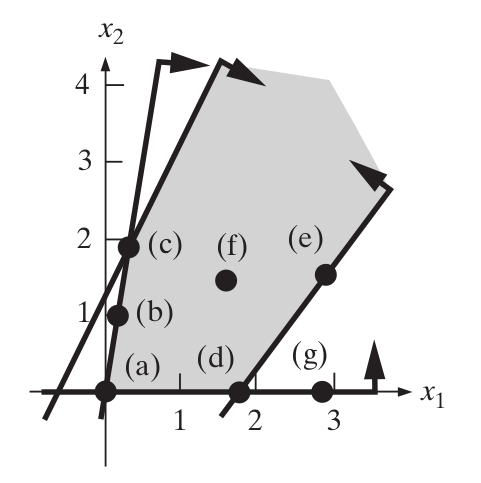
\includegraphics[width=\linewidth]{points_classification.png}
      \end{center}
    \end{column}
    \begin{column}{.45\textwidth}
      (a), (c), and (d) are both extreme points and boundary points. \\
      (b) and (e) are boundary points that are not extreme. \\
      (f) is interior because no constraint is active. \\
      (g) is neither interior nor boundary (nor extreme) because it is infeasible.\cite{rardin}
    \end{column}
  \end{columns}
\end{frame}


\begin{frame}{The standard form}

  \begin{block}{Standard form}
    For a LP with $n$ variables and $m$ constraints, the standard form is given by:
    \begin{equation*}
      \begin{aligned}
        \text{maximize } \quad & z = c_1x_1+c_2x_2 +\cdots + c_nx_n \\
        \text{subject to }\quad &
        \begin{array}{rcl}
          a_{11}x_1+a_{12}x_2+\cdots+a_{1n}x_n &= &b_1 \\
          a_{21}x_1+a_{22}x_2+\cdots+a_{2n}x_n &= &b_2 \\
          \vdots &=& \vdots\\
          a_{m1}x_1+a_{m2}x_2+\cdots+a_{mn}x_n &= &b_m \\
        \end{array}
      \end{aligned}
    \end{equation*}
    where $x_1,\ldots,x_n\geq0$ and $b_1,\ldots,b_m\geq0$
  \end{block}

Thus:
\begin{equation*}
  \begin{aligned}
    \text{maximize } \quad & z = cx \\
    \text{subject to }\quad &
    \begin{array}{c}
      Ax=b\\
      x\geq0\\
      b\geq0
    \end{array}
  \end{aligned}
\end{equation*}

\end{frame}

\begin{frame}
Of course, not always the system is proposed in this standard form, so\cite{carter}:
\begin{itemize}
  \item We need to leave a maximization problem. If the problem is to minimize the objective function, we simply multiply it by $(-1)$.
  \item In order to change inequality constraints into equality constraints we use {\it slack} variables for $\leq$ inequalities:
  \[
  3x_1+4x_2 \leq 7  \rightarrow  3x_1+4x_2+s_1 =7
  \]
  or {\it surplus} variables for $\geq$ inequalities:
  \[
  x_1+3x_2\geq 10 \rightarrow x_1+3x_2 -s_2 =10
  \]
  \item All variables should be non-negative. If some variable $x_1$ needs to be considered as unrestricted in sign, we will replace it by $x_1'-x_1''$, with $x_1',x_1''\geq 0$
\end{itemize}
\end{frame}

\subsection{The algebra behind the standard form}

\begin{frame}
  \begin{itemize}
 \item The system of linear equations, $Ax = b$, consists of $m$ equations and $n$
unknowns (the original decision variables plus the rest introduced to get a standard form). If the system has any solution, then $m \leq n$.
\item If $m = n$ (and if $rank (A) = m$ and $A$ is nonsingular), then 
$x = A^{-1}b$. No optimization needed!
\item If $m < n$, there are infinitely many solutions and $n -m$ degrees of freedom. 
\item A {\bf basic solution} is obtained by setting $n - m$ of the variables to zero ({\bf non-basic variables}), and solving for the remaining ({\bf basic}) $m$ variables. The number of basic solutions is $\binom{n}{n-m}=\binom{n}{m}=\frac{n!}{m!(n-m)!}$
\item Basic solutions that do not satisfy all problem constraints and non-negativity constraints are {\bf infeasible solutions}.
\item An {\bf optimal basic feasible solution} is a
basic feasible solution that optimizes the objective function. 
\end{itemize}
\end{frame}

\subsection{The Simplex algorithm}

\begin{frame}
We define
two extreme points of the feasible region (or two basic feasible solutions) as being adjacent if all but one of their basic variables are the same. Thus, {\em a transition from one basic
feasible solution to an adjacent basic feasible solution can be thought of as exchanging
the roles of one basic variable and one non-basic variable}. The Simplex method performs a sequence of such transitions and thereby examines a succession of adjacent
extreme points. A transition to an adjacent extreme point will be made only if by doing
so the objective function is improved (or stays the same). It is a property of linear programming problems that this type of search will lead us to the discovery of an optimal
solution (if one exists). The Simplex method is not only successful in this sense, but it
is remarkably efficient because it succeeds after examining only a fraction of the basic
feasible solutions.\cite{carter}
\end{frame}

\begin{frame}
The algorithm consists in:
\begin{enumerate}
  \item obtaining an initial feasible
solution,
\item make transitions to a better basic feasible solution,
\item recognizing an optimal solution.
\end{enumerate}
From any basic feasible solution, we have the assurance
that, if a better solution exists at all, then there is an adjacent solution that is better than the
current one.\cite{carter}
\end{frame}

\begin{frame}{The algorithm}
\begin{enumerate}
  \item Convert the system of inequalities to equations (using slack or surplus variables).
  \item Set the objective function $z$ to zero.
  \item Create the Simplex tableau and label active and basic variables.
  \item Select the pivot column (the one with the most negative coefficient in the zeroed objective function). Linked to the {\bf entering variable}.
  \item Select the pivot row (once divided the entry in the constant column by the ceffient in that row in the pivot column, we choose the smallest ratio). Linked to the {\bf leaving variable}.
  \item The pivot is the intersection between the pivot row and pivot column.
  \item Use the pivot value to make zeros in the rest of elements in the column.
  \item Repeat the process from step 4, until the $z$ row is all non-negative.
\end{enumerate}

\end{frame}

\begin{frame}{Example. Standard form}


  \begin{equation*}
    \begin{aligned}
      \text{maximize } \quad & z = 8x_1+5x_2 \\
      \text{subject to }\quad &
      \begin{array}{rcl}
        x_1 &\leq &150 \\
        x_2 &\leq &250 \\
        2x_1+x_2 &\leq &500 \\
        x_1,x_2 &\geq& 0
      \end{array}
    \end{aligned}
  \end{equation*}
We build first the standard form:
\begin{eqnarray*}
  -8x_1-5x_2-0s-0t-0u+z&=&0\\
  x_1+s&=&150\\
  x_2+t&=&250\\
  2x_1+x_2+u&=&500
\end{eqnarray*}
\end{frame}

\begin{frame}{Example. The Simplex Tableau}
  We write the coefficients matrix and we identify the basic ($m=3$) and non-basic ($n-m=5-3=2$ degrees of freedom) variables:
  \begin{equation}
\begin{array}{cc}
&\\
&z \\
\rightarrow &s \\
&t \\
&u\\
\mathrm{basic}
\end{array}
%
\begin{array}{c|ccccc|c}
  z & x_1 & x_2 & s & t & u & b \\ \hline
  1 & -8 & -5 & 0 & 0 & 0 & 0 \\ \hline
  0 & 1 & 0 & 1 & 0 & 0 & 150  \\
  0 & 0 & 1 & 0 & 1 & 0 & 250 \\
  0 & 2 & 1 & 0 & 0 & 1 & 500 \\
    & \uparrow & & & & &
\end{array}
%\end{matrix}
\end{equation}
  Note that the basic variables are those for which each column is a collection of 1 and zero. We will arbitrarily assign zeros to the non-basic variables.
So a possible solution is $\boxed{P_A=(x_1=0, x_2=0)\Rightarrow z=0}$.

  The arrow marks the pivot column. We will take the pivot row by considering which is the lowest value among 150/1 and 500/2. So, the pivot row corresponds to the $s$ basic variable.
\end{frame}

% \begin{frame}{Example. Graphic solution}
%   \begin{center}
%    \includegraphics[width=0.5\linewidth]{LP7.pdf}
%   \end{center}
% \end{frame}

\begin{frame}{Example. Entering/leaving variables}

\begin{equation*}
\begin{array}{cc}
&\\
R_1+8R_2&z \\
&x_1 \\
&t \\
\rightarrow R_4-2R_2&u\\
&\mathrm{basic} \\
\end{array}
\begin{array}{c|ccccc|c}
  z & x_1 & x_2 & s & t & u & b \\ \hline
  1 & 0 & -5 & 8 & 0 & 0 & 1200 \\ \hline
  0 & 1 & 0 & 1 & 0 & 0 & 150  \\
  0 & 0 & 1 & 0 & 1 & 0 & 250 \\
  0 & 0 & 1 & -2 & 0 & 1 & 200 \\
    &  & \uparrow& & & &
\end{array}
\end{equation*}
$P_B=(150,0)$ and $z(P_B)=1200$ with $t=250$, $u=200$, $s=0$.
\end{frame}

\begin{frame}
\begin{equation*}
\begin{array}{cc}
&\\
R_1+5R_4&z \\
&x_1 \\
\rightarrow R_3-R_4&t \\
&x_2\\
&\mathrm{basic} \\
\end{array}
\begin{array}{c|ccccc|c}
  z & x_1 & x_2 & s & t & u & b \\ \hline
  1 & 0 & 0 & -2 & 0 & 5 & 2200 \\ \hline
  0 & 1 & 0 & 1 & 0 & -1 & 150  \\
  0 & 0 & 0 & 2 & 0 & 1 & 50 \\
  0 & 0 & 1 & -2 & 0 & 1 & 200 \\
    &  & & \uparrow& & &
\end{array}
\end{equation*}

\begin{equation*}
\begin{array}{cc}
&\\
R_1+5R_4&z \\
&x_1 \\
\rightarrow R_3-R_4&s \\
&x_2\\
&\mathrm{basic} \\
\end{array}
\begin{array}{c|ccccc|c}
  z & x_1 & x_2 & s & t & u & b \\ \hline
  1 & 0 & 0 & 0 & 1 & 4 & 2250 \\ \hline
  0 & 1 & 0 & 0 & -1/2 & 1/2 & 125  \\
  0 & 0 & 0 & 1 & 1/2 & -1/2 & 25 \\
  0 & 1 & 0 & 1 & 0 & 0 & 250 \\
    &  & & \uparrow& & &
\end{array}
\end{equation*}

$\boxed{P_D=(125,250)}$ and $\boxed{z(P_D)=2250}$ with $t,u=0$ (binding constraints), $s=25$ (non-binding constraint).
\end{frame}


\begin{frame}
  \begin{center}
    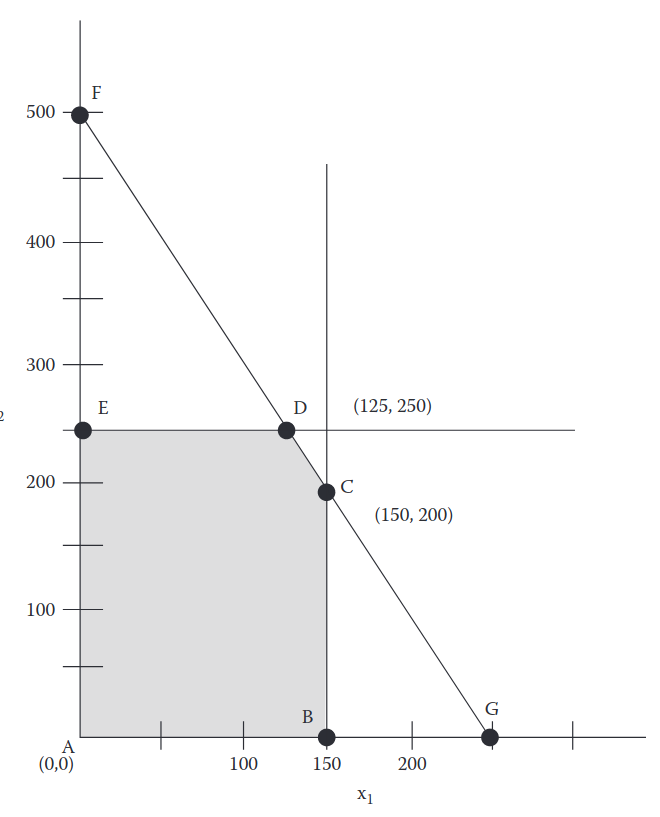
\includegraphics[width=0.4\linewidth]{simplex_example.png}
  \end{center}
  Simplex steps for the given example (taken from \cite{carter}).
\end{frame}

\begin{frame}{Exercises}
  Solve, using the Simplex method, the Exercises 3 through 7 of the previous session. Check also \href{https://realpython.com/linear-programming-python/}{different methods} for optimizing LP problems in python.
\end{frame}

\subsection{Initial solutions for General Constraints}

\begin{frame}{Artificial variables}

  When adding slack variables, we end up finding an initial feasible set of basic variables. But what happens when not all constraints are of the form "$\leq$"?\cite{carter}

  \begin{enumerate}
    \item Make all right hand sides $b_i$ of the constraint (in)equalities positive. If they are not, multiply the expression by $(-1)$.
    \item If we end up just with slack variables, they can be directly used as initial basic variables. If the expressions are of the type $\geq$ the selection of initial basic variables is not trivial.
    \item We then create {\bf artificial variables}, as a trick to create a starting basic solution
  \end{enumerate}
  \begin{equation*}
    \begin{aligned}
      \text{maximize } \quad & z = x_1+3x_2 \\
      \text{subject to }\quad &
      \begin{array}{rcl}
        2x_1 -x_2 &\leq &-1 \\
        x_1+x_2 &= &3 \\
        x_1,x_2 &\geq& 0
      \end{array}
    \end{aligned}
  \end{equation*}
\end{frame}

\begin{frame}
  By leaving the right hand side of the constraints positive and adding a surplus variable, we end up having
  \begin{equation*}
    \begin{aligned}
       \text{subject to }\quad &
      \begin{array}{rcl}
        -2x_1 +x_2 -s_1 &= &1 \\
        x_1+x_2 &= &3
      \end{array}
    \end{aligned}
  \end{equation*}
  and now we introduce the artificial variables to create an initial solution:
  \begin{equation*}
    \begin{aligned}
       \text{subject to }\quad &
      \begin{array}{rcl}
        -2x_1 +x_2 -s_1 +R_1&= &1 \\
        x_1+x_2 +R_2&= &3
      \end{array}
    \end{aligned}
  \end{equation*}
  with all variables non-negative. Recall that, in fact, $R_1=R_2=0$, so they will be just used temporarily.
  \\[10pt]

  There are two main methods to solve the problem: the two-phase method, explained next, and the \href{https://www.youtube.com/watch?v=btjxqq-vMOg}{big-M method}, that we are not explaining here.
\end{frame}

\begin{frame}[allowframebreaks]{The Two-Phase method}

  \begin{enumerate}
    \item First we will use the Simplex method to minimize the values of $R_1$ and $R_2$. 
    \item If they reach the value of zero, there is a solution for the original problem. If not, there is no feasible solution to the original problem.
  \end{enumerate}
  In the above example, we want to minimize the function $z_R=R_1+R_2$ or, what is the same, we want to maximize the function $z_R=-R_1-R_2$
  \begin{equation*}
    \begin{array}{c}
    \\
    z_R\\
    R_1\\
    R_2\\
    \end{array}
    \begin{array}{ccccc|c}
       x_1 & x_2 & s_1 & R_1 & R_2 & Solution \\ \hline
       0 & 0 & 0 & 1 & 1 & 0 \\ \hline
       -2 & 1 & -1 & 1 & 0 & 1  \\
       1 & 1 & 0 & 0 & 1 & 3 \\
    \end{array}
    \end{equation*}

  Next, we transform the problem in order to get  basic variables (columns of one 1 and the rest zeros). For example, by using the second and third row to make appear 0 in the first row for the artificial variables:
  \begin{equation*}
    \begin{array}{c}
    \\
    z_R\\
    R_1\\
    R_2\\
    \end{array}
    \begin{array}{ccccc|c}
       x_1 & x_2 & s_1 & R_1 & R_2 & Solution \\ \hline
       1 & -2 & 1 & 0 & 0 & -4 \\ \hline
       -2 & 1 & -1 & 1 & 0 & 1  \\
       1 & 1 & 0 & 0 & 1 & 3 \\
    \end{array}
  \end{equation*}
  We can solve this problem with the Simplex method, obtaining a tableau:
  \begin{equation*}
    \begin{array}{c}
    \\
    z_R\\
    x_2\\
    x_1\\
    \end{array}
    \begin{array}{ccccc|c}
       x_1 & x_2 & s_1 & R_1 & R_2 & Solution \\ \hline
       0 & 0 & 0 & 1 & 1 & 0 \\ \hline
       0 & 1 & -1/3 & 1/3 & 2/3 & 7/3  \\
       1 & 0 & 1/3 & -1/3 & 1/3 & 2/3 \\
    \end{array}
  \end{equation*}
    which provides the optimal solution for Phase 1. This means that the original problem has solution (as $R_1=R_2=0$). In Phase 2, we will replace the first row by the original maximization problem and leave out the artificial variables, solving the now standard Simplex problem:
    \begin{equation*}
      \begin{array}{c}
        \\
        z\\
        x_2\\
        x_1\\
      \end{array}
      \begin{array}{ccc|c}
        x_1 & x_2 & s_1 &  Solution \\ \hline
        -1 & -3 & 0 &  0 \\ \hline
        0 & 1 & -1/3 & 7/3  \\
        1 & 0 & 1/3  & 2/3 \\
      \end{array}
    \end{equation*}
    that leads to
    \begin{equation*}
      \begin{array}{c}
        \\
        z\\
        x_2\\
        s_1\\
      \end{array}
      \begin{array}{ccc|c}
        x_1 & x_2 & s_1 &  Solution \\ \hline
        2 & 0 & 0 &  9 \\ \hline
        1 & 1 & 0 & 3  \\
        3 & 0 & 1  & 2 \\
      \end{array}
    \end{equation*}

      Draw the graphical solution of this problem and interpret the results.

  \end{frame}

  \begin{frame}{Information in the tableau}
    Some special cases:
    \begin{description}
      \item[Multiple optimal solutions] If a zero appears in the objective function row corresponding to a non-basic
      variable, then that non-basic variable can enter the basis without changing the value of
      the objective function. So, two adjacent points have the same objective function value.
      \item[Unbounded solution] If in any tableau the constraint coefficients corresponding to a non-basic variable are all
      either negative or zero, then that non-basic variable can be increased arbitrarily without
      violating any constraint. Thus, the feasible region is unbounded in the direction of that
      variable.
      \item[Degenerate solutions] A solution to a linear programming problem is said to be degenerate if one or more of the
      basic variables has a value of zero. This shows redundancy in the constraints.
    \end{description}
  \end{frame}

\subsection{Application of SIMPLEX to non-linear problems}


\begin{frame}{Application of SIMPLEX to non-linear problems}
  Algorithm (see example in the next page):
\begin{enumerate}
\item In $\mathbf{R}^2$, we form a triangle with vertices at $x^{[0]}$ and the two points $x^{[1]} = x^{[0]} + l_1e^{[1]}$ and  $x^{[2]} = x^{[0]} + l_2e^{[2]}$. In $\mathbf{R}^N$ the triangle becomes a simplex with $N + 1$ vertices.
\item We aim at moving ${x^{[0]}, x^{[1]}, x^{[2]},...}$ so that the triangle comes to enclose a local minimum $x_{\mathrm{min}}$ while shrinking in size.  First, the vertex of highest cost function value is moved in the direction of the {\bf triangle’s center} towards a region where we expect the cost function values to be lower. After a sequence of such moves, the triangle eventually contains in its interior a local minimum. 
\item The size of the triangle is progressively reduced until it tightly bounds the local minimum, as the vertex moves are most likely to succeed when the triangle is small enough that $F(x)$ varies linearly over the triangle region.
\end{enumerate}
\end{frame}

\begin{frame}
  \begin{center}
    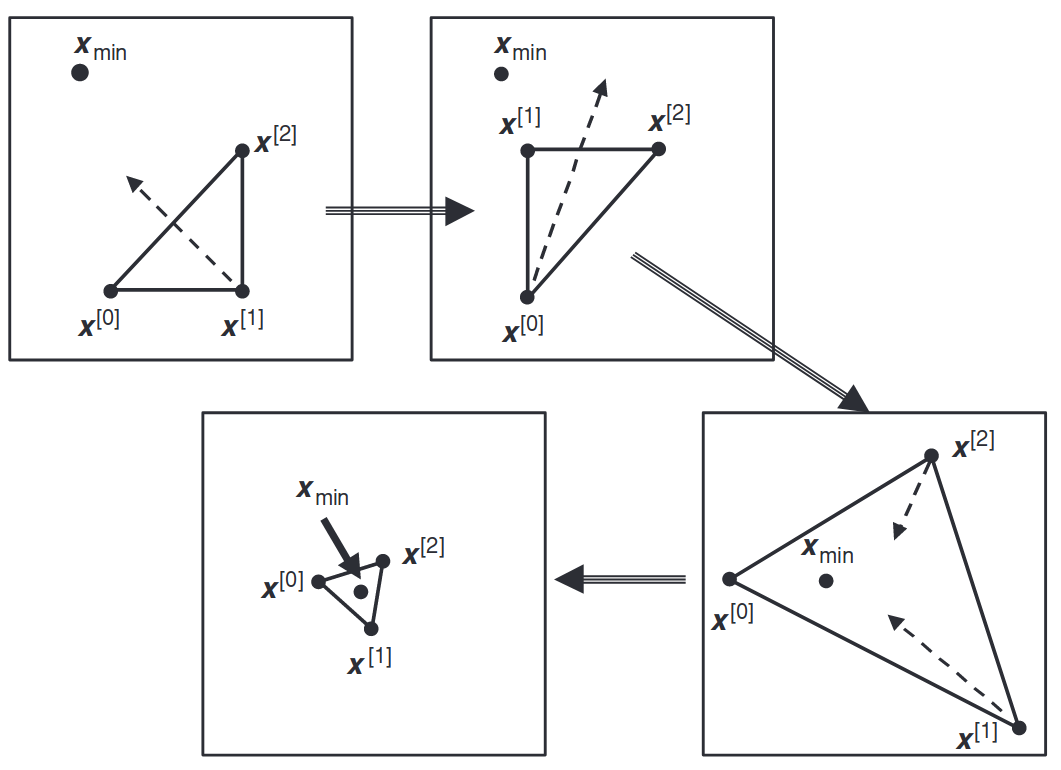
\includegraphics[width=0.7\linewidth]{simplex_nonlinear.png}
  \end{center}
  The simplex method moves the vertices of the simplex (in two dimensions, a triangle) until it contains the local minimum, and shrinks the simplex to find the local minimum (taken from \cite{beers}).
\end{frame}

\section{Duality}


\begin{frame}
\frametitle{Learning outcomes}
\begin{itemize}
  \item Understanding Dual and Primal problems in LP
  \item Economic interpretation
  \item Conditions of optimality
  \item Resolution of the dual by the primal and penalty method
\end{itemize}
\end{frame}

\note{\url{https://www.youtube.com/watch?v=yU8updOR87c}}
\begin{frame}[allowframebreaks]{A first example}

  Linear programming problems come in pairs!

  \begin{equation*}
    \begin{aligned}
      \text{maximize  } \quad & 4x_1 + x_2 +5x_3 +3x_4 \\
      \text{subject to }\quad &
      \left\{
      \begin{array}{rcl}
        x_1 - x_2 -x_3 +3x_4 &\leq &1 \\
        5x_1 + x_2 +3x_3 +8x_4 &\leq &55 \\
        -x_1 + x_2 +3x_3 -5x_4 &\leq &3 \\
        x_1,x_2,x_3 &\geq& 0
      \end{array}
      \right.
    \end{aligned}
  \end{equation*}

note that
\begin{eqnarray*}
  y_1(x_1 - x_2 -x_3 +3x_4)&+&\\y_2(5x_1 + x_2 +3x_3 +8x_4)&+&\\y_3(-x_1 + x_2 +3x_3 -5x_4) &\leq& y_1+55y_2+3y_3
\end{eqnarray*}

\end{frame}
\begin{frame}{Primal and Dual}

We see that maximizing the {\bf Primal objective function} $4x_1 + x_2 +5x_3 +3x_4$ is
  equivalent to minimize the {\bf Dual objective function} $y_1+55y_2+3y_3$:

    \begin{equation*}
    \begin{aligned}
      \text{minimize } \quad & y_1+55y_2+3y_3 \\
      \text{subject to }\quad &
      \left\{
      \begin{array}{rcl}
        y_1 + 5y_2 -y_3 &\geq &4 \\
        -y_1 +y_2 +y_3 &\geq &1 \\
        -y_1 +3y_2 +3y_3 &\geq &5 \\
        3y_1 +8y_2 -5y_3 &\geq &3 \\
        y_1,y_2,y_3,y_4 &\geq& 0
      \end{array}
      \right.
    \end{aligned}
  \end{equation*}

  \end{frame}


\begin{frame}{Generalization}
In general, if we can write the LP problem in its {\bf normal formulation}:
\[
\begin{rcases}
\text{min }\quad\uvec{c}^t \uvec{x}\\
\text{subject to }\quad A\uvec{x}\geq \uvec{b}, \forall x_i\geq0
\end{rcases} \text{PRIMAL}
\]

\[
\begin{rcases}
\text{max }\quad\uvec{b}^t \uvec{y}\\
\text{subject to }\quad A^t\uvec{y}\leq \uvec{c}, \forall y_i\geq0
\end{rcases} \text{DUAL}
\]
The dual problem is a transposition of the primal problem. Since any LP can be written in the standard form
above, any LP has a dual.
\end{frame}

\begin{frame}{Problem transformations}
  \begin{enumerate}
    \item if you are asked to minimize $f(x)$, this is equivalent to maximize $-f(x)$;
    \item add slack/surplus variables if you want to transform an inequality into an equality contraint;
    \item $a\cdot x=b$ is equivalent to having, simultaneously, $a \cdot x \leq b$ and $a \cdot x \geq b$;
    \item replace an unconstrained variable $x_i$ by $u_i-v_i$ and impose that $u_i,v_i \geq 0$
  \end{enumerate}
  Trick: Leave equality constraints to use the simplex algorithm. Use the inequality constraints for the duality theorem to be used.
\end{frame}

\begin{frame}{}
\begin{Exercise}
  Find the dual problem of
  \begin{equation*}
  \begin{aligned}
    \text{maximize } \quad & 3x_1 +2x_2 \\
    \text{subject to }\quad &
    \left\{
    \begin{array}{rcl}
      2x_1+x_2 &\leq &4 \\
      2x_1+3x_2 &\leq &6 \\
      x_1,x_2 &\geq& 0
    \end{array}
    \right.
  \end{aligned}
\end{equation*}
Solve it graphically and using Simplex. 
\end{Exercise}
\end{frame}

\note{\begin{center}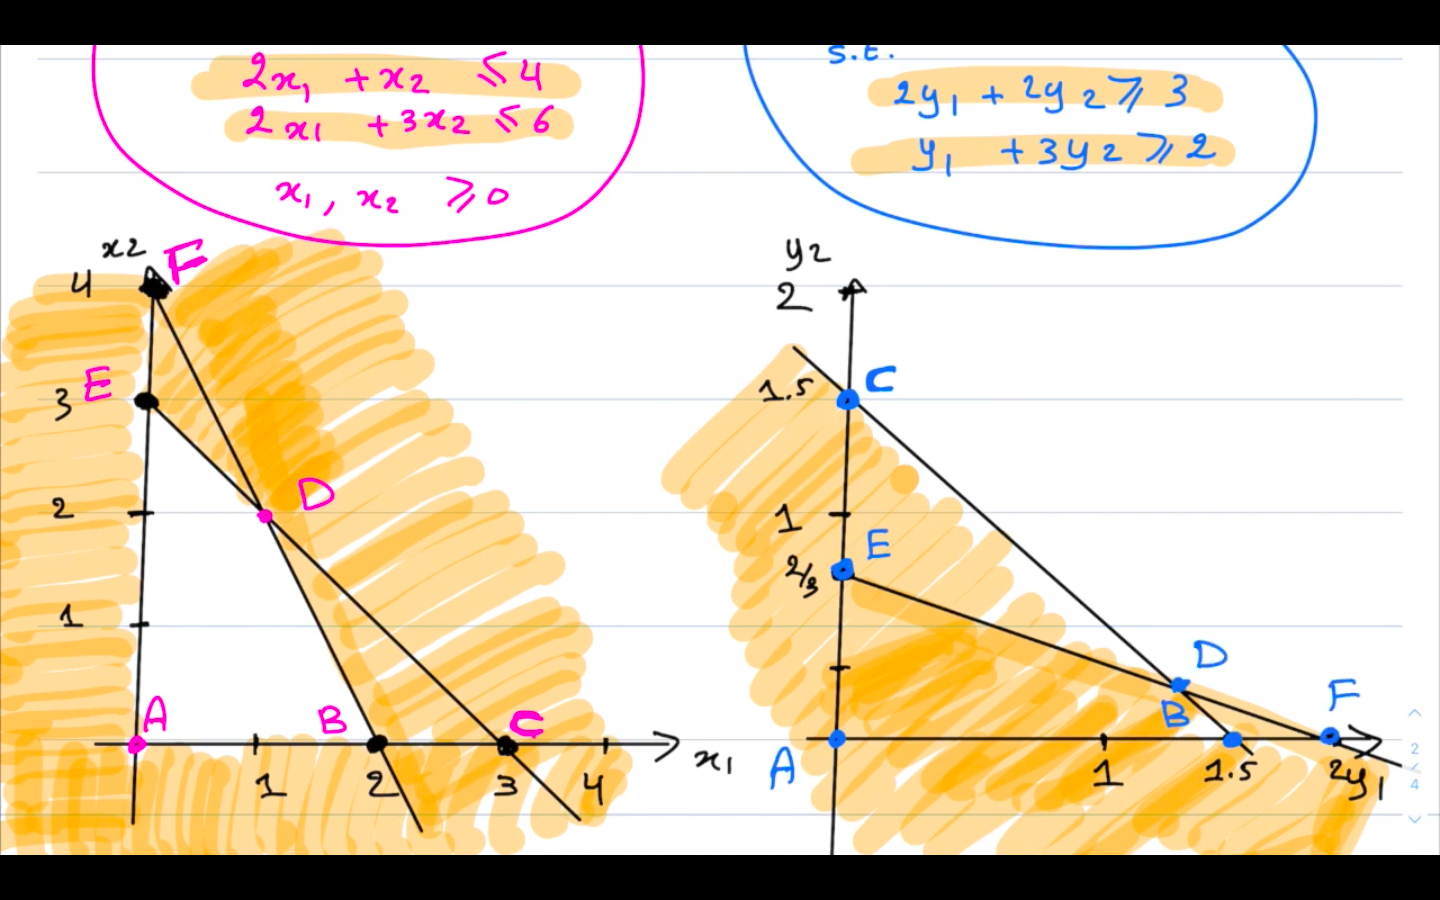
\includegraphics[width=0.8\linewidth]{answer1.png}\end{center}}
\note{\begin{center}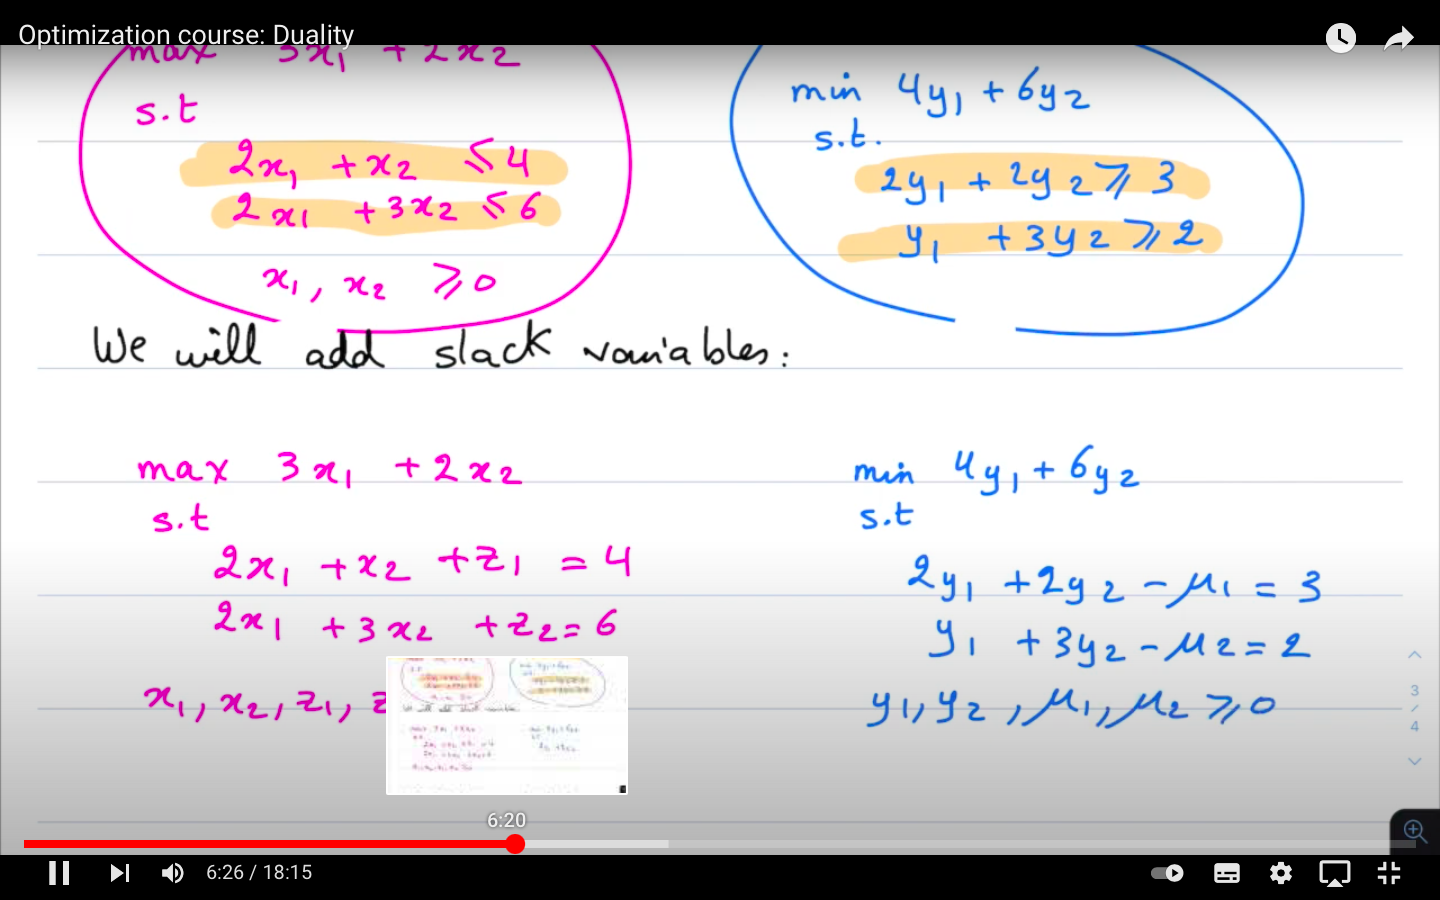
\includegraphics[width=0.8\linewidth]{answer3.png}\end{center}}
\note{\begin{center}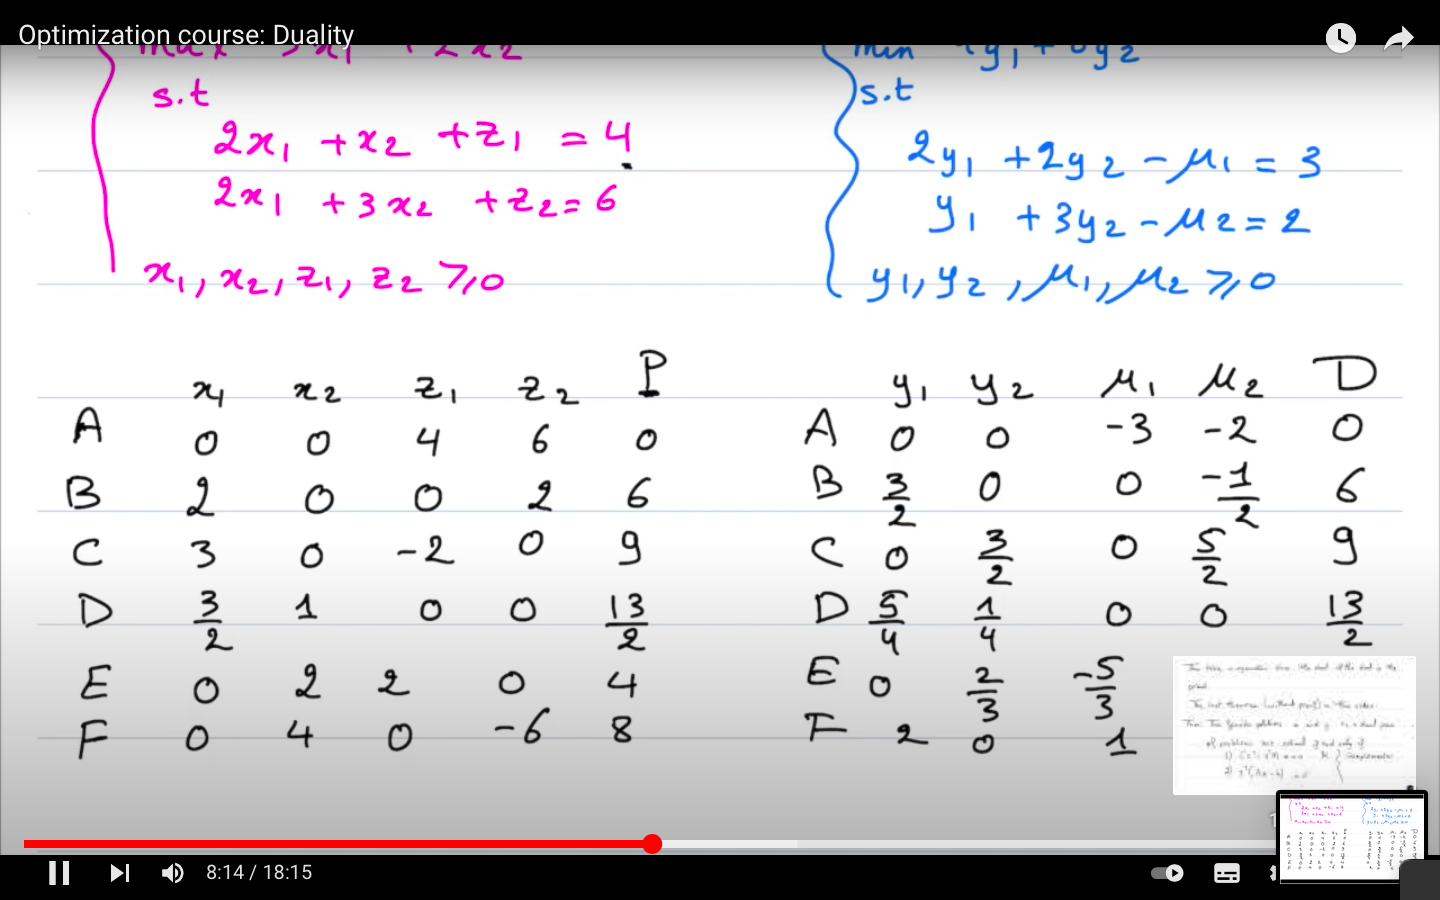
\includegraphics[width=0.8\linewidth]{answer2.png}\end{center}}
\note{\begin{center}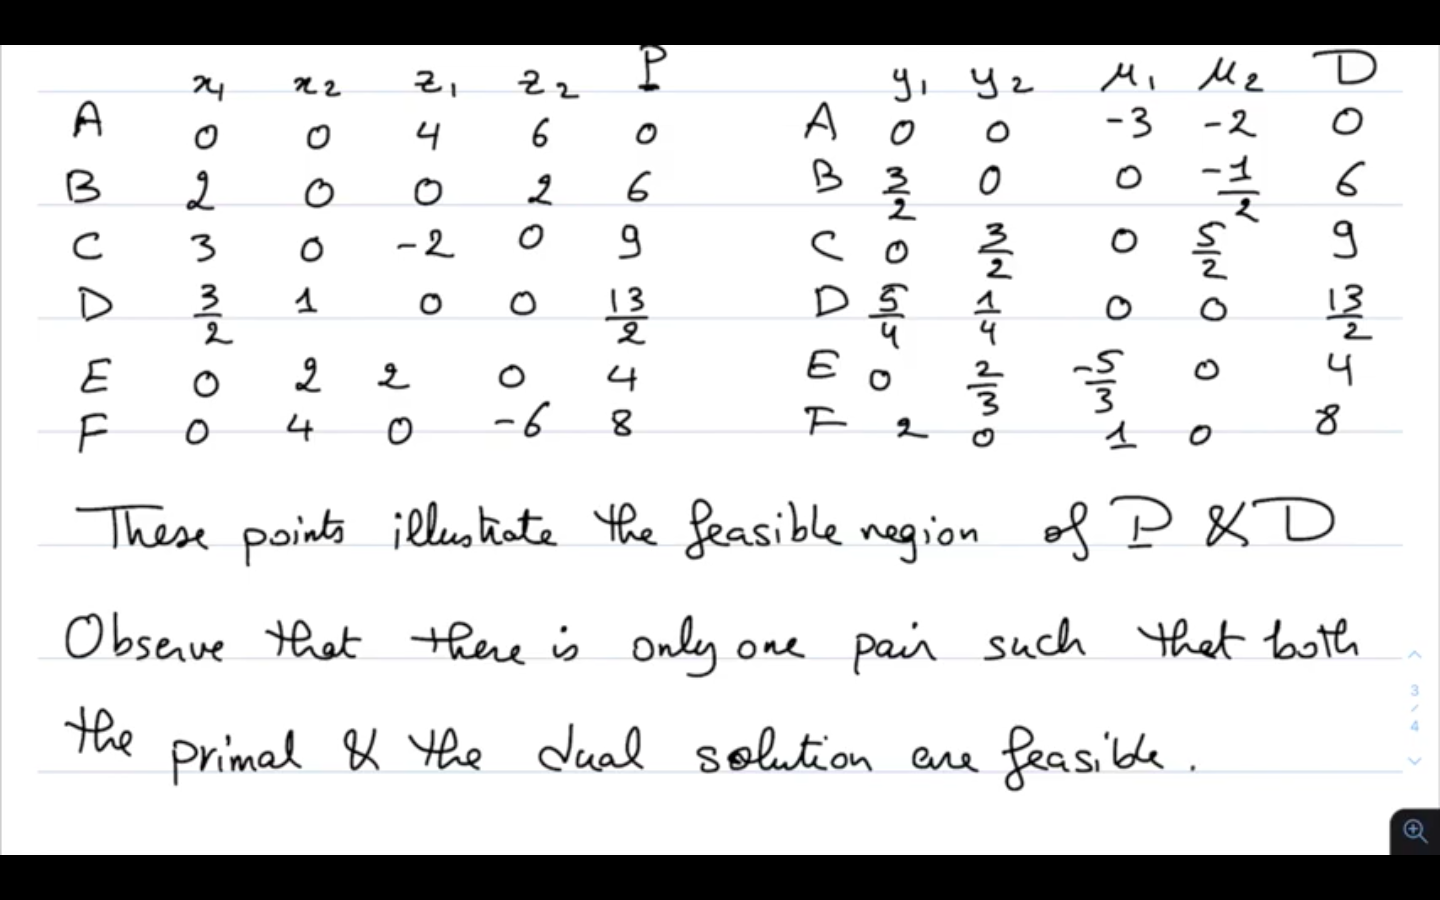
\includegraphics[width=0.8\linewidth]{answer4.png}\end{center}}

\begin{frame}{}
\begin{Exercise}
  Find the dual problem of
  \begin{equation*}
  \begin{aligned}
    \text{minimize } \quad & 4x_1 +4x_2+x_3 \\
    \text{subject to }\quad &
    \left\{
    \begin{array}{rcl}
      x_1+x_2+x_3 &\leq &2 \\
      2x_1+x_2 &= &3 \\
      2x_1+x_2+3x_3 &\geq &3 \\
      x_1,x_2,x_3 &\geq& 0
    \end{array}
    \right.
  \end{aligned}
\end{equation*}
Trick: normalize the problem first: eg $2x_1+x_2=3 \rightarrow \begin{cases}2x_1+x_2 \geq 3\\2x_1+x_2\leq 3\end{cases}$.
\end{Exercise}
\end{frame}
\note{
\url{https://www.youtube.com/watch?v=wVnr1HhUCT0}
}

\subsection{Some theory}

\begin{frame}{Dual of the dual}
\begin{theorem}
  In the case of linear programming, the dual of the dual is the primal.
\end{theorem}
\begin{proof}
 \[
\begin{rcases}
\text{max }\quad\uvec{b}^t \uvec{y}\\
\text{subject to }\quad A^t\uvec{y}\leq \uvec{c}, \forall y_i\geq0
\end{rcases} \text{PRIMAL}
\]
is equivalent to
\[
\begin{rcases}
\text{min }\quad-\uvec{b}^t \uvec{y}\\
\text{subject to }\quad -A^t\uvec{y}\geq -\uvec{c}, \forall y_i\geq0
\end{rcases} \text{DUAL}
\]
where, by taking again the Dual, leads to the original Primal.
\end{proof}
\end{frame}

\begin{frame}[allowframebreaks]{Meaning of Duality}
  Let us retake the example we saw in the last session:

  \begin{equation*}
    \begin{aligned}
      \text{maximize } \quad & z = 8x_1+5x_2 \\
      \text{subject to }\quad &
      \begin{array}{rcl}
        x_1 &\leq &150 \\
        x_2 &\leq &250 \\
        2x_1+x_2 &\leq &500 \\
        x_1,x_2 &\geq& 0
      \end{array}
    \end{aligned}
  \end{equation*}

  We found out that, from the initial tableau:

\begin{equation*}
\begin{array}{cc}
&\\
&z \\
\rightarrow &s \\
&t \\
&u\\
\mathrm{basic}
\end{array}
%
\begin{array}{c|ccccc|c}
  z & x_1 & x_2 & s & t & u & b \\ \hline
  1 & -8 & -5 & 0 & 0 & 0 & 0 \\ \hline
  0 & 1 & 0 & 1 & 0 & 0 & 150  \\
  0 & 0 & 1 & 0 & 1 & 0 & 250 \\
  0 & 2 & 1 & 0 & 0 & 1 & 500 \\
    & \uparrow & & & & &
\end{array}
%\end{matrix}
\end{equation*}

and after applying the different steps of the Simplex method we ended up with the final tableau:

  \begin{equation*}
  \begin{array}{cc}
  &\\
  R_1+5R_4&z \\
  &x_1 \\
  \rightarrow R_3-R_4&s \\
  &x_2\\
  &\mathrm{basic} \\
  \end{array}
  \begin{array}{c|ccccc|c}
    z & x_1 & x_2 & s & t & u & b \\ \hline
    1 & 0 & 0 & 0 & 1 & 4 & 2250 \\ \hline
    0 & 1 & 0 & 0 & -1/2 & 1/2 & 125  \\
    0 & 0 & 0 & 1 & 1/2 & -1/2 & 25 \\
    0 & 1 & 1 & 0 & 0 & 0 & 250 
  \end{array}
  \end{equation*}

Now, if we multiply the original availability of each resource (shown in the original tableau) by its marginal worth (taken from the final tableau) and get the sum, we obtain the optimal objective function value:

\[
z* = 2250 = 0(150)+1(250)+4(500)
\]

\end{frame}

\begin{frame}{Duality properties}


\begin{theorem}[Weak Duality]
  In a max LP, the value of primal objective function for any feasible solution is bounded from above by any feasible solution to its dual:
  \[\bar{z} \leq \bar{w} \]
  \label{the:weak}
\end{theorem}
The statement is analogous to a minimization problem.
\begin{theorem}[Unboundness property]
  If primal (dual) problem has an unbounded solution, then the dual (primal) is unfeasible.
  \[\bar{z} \leq \infty \]
\end{theorem}
\end{frame}

\begin{frame}[allowframebreaks]{Duality properties}


\begin{theorem}[Strong Duality]
  If the primal problem has an optimal solution,
  \[
  x^* = (x_1^*, \ldots, x_n^*)
  \]
  then the dual also has an optimal solution,
  \[
  y^* = (y_1^*, \ldots, y_m^*)
  \]
and
\[
z^* := \sum_j c_j x_j^* = \sum_i b_i y_i^* := w^*
\]
\label{the:strong}
\end{theorem}
Thus: if feasible objective function values are found for a primal and dual pair of problems, and if these values are equal to each other, then both of the solutions are optimal solutions.

The Shadow prices that appear at the top of the optimal tableau of the primal problem are precisely the optimal values of the dual variables!
\end{frame}

\begin{frame}{A useful table}
  For any two given LP problems:
\begin{table}
  \begin{tabular}{c|c|c|c}
    Primal / Dual & not feasible & unbounded  & has a solution \\\hline
    not feasible & possible & possible & no \\\hline
    unbounded & possible & no & no \\\hline
    has a solution & no & no & same values\\
  \end{tabular}
\end{table}
The simplex algorithm solves the primal and dual problems simultaneously.
\end{frame}

\begin{frame}{Cases with no optimal solutions for primal and dual}
  Exactly one of the following mutually exclusive cases always occurs:
  \begin{itemize}
    \item Both primal and dual problems are feasible, and both have optimal (and equal) solutions.
    \item Both primal and dual problems are infeasible (have no feasible solution).
    \item The primal problem is feasible but unbounded, and the dual problem is infeasible.
    \item The dual problem is feasible but unbounded, and the primal problem is infeasible.
  \end{itemize}
\end{frame}

\subsection{Complementary slackness}

\begin{frame}[allowframebreaks]{Complementary slackness}
  Because each decision variable in a primal problem is associated with a constraint in the dual problem, each such variable is also associated with a slack or surplus variable in the dual.

  {\bf Variables in one problem are complementary to constraints in the other.}

  In any solution, if the primal variable is basic (with value $\geq0$, hence having slack, hence being non-binding), then the associated dual variable is non-basic ($=0$, hence having no slack, hence being binding), and viceversa.


  \begin{theorem}[Complementary slackness]
    If in an optimal solution to a LP problem an inequality constraint is not binding, then the dual variable corresponding to that constraint has a value of zero in any optimal solution to the dual problem. 
    \label{the:CST}
  \end{theorem}

  \framebreak

  Let us see how this can be better understood. Let us take a general primal/dual case
  \[
\begin{rcases}
\text{max }\quad\uvec{c}^t \uvec{x}\\
\text{subject to }\quad A\uvec{x}\leq \uvec{b}, \forall x_i\geq0
\end{rcases} \text{PRIMAL}
\]

\[
\begin{rcases}
\text{min }\quad\uvec{b}^t \uvec{y}\\
\text{subject to }\quad A^t\uvec{y}\geq \uvec{c}, \forall y_i\geq0
\end{rcases} \text{DUAL}
\]

  \framebreak

  Let vectors $x_0,y_0$ be feasible solutions for the $(max)$ and the $(min)$ problems, respectively. The weak duality theorem \ref{the:weak} states that (we remove the transpose where it is obvious, for simplicity)
  \[\text{max} \quad c\cdot x_0 \leq \text{min}\quad b\cdot y_0\]

  Then we can say that (we will not demonstrate it here)
  \[b\cdot y_0 - c\cdot x_0 = \underbrace{(b-Ax_0)}_u\cdot y_0+\underbrace{(A^ty_0-c)}_v\cdot x_0\]
  
  where $u$ is the vector of slack variables in the primal problem and $v$ is the vector of the slack variables in the dual.

  \framebreak

  According to Theorem \ref{the:strong}, when $x_0,y_0=x^*,y^*$ are optimal solutions, \[b\cdot y^* - c\cdot x^* =0\]
  This means that in such optimal solutions
  \[\underbrace{(b-Ax^*)}_{u\geq 0}\cdot y^*+\underbrace{(A^ty^*-c)}_{v\geq 0}\cdot x^*=0\]
  The fact that all terms are nonnegative implies that 
  \begin{equation}(b-Ax^*)\cdot y^*=(A^ty^*-c)\cdot x^*=0\label{eq:dual}\end{equation}
  \framebreak

  Now let us haver a look at one of these terms:
  \[(b-Ax^*)\cdot y^*\equiv u\cdot y^*=0\]
  As the components of the two vectors are nonnegative aswell: $u_1,\ldots,u_m\geq0$ and $y^*_1,\ldots,y^*_m\geq0$, 
  \[\underbrace{u_1 y_1^*}_{\geq0}+\cdots \underbrace{u_m y_m^*}_{\geq0}=0\]
  So, each term should be zero!. Now, for each $i=1,\ldots,m$ we must have at least one of $u_i,y_i^*=0$. So, if $u_i\neq 0 \Rightarrow y_i^*=0$ and the other way around. The same occurs to the other term in Eq.\ref{eq:dual}.
  
  \framebreak 

  Thus, Theorem \ref{the:CST} can be reformulated as:
  \begin{theorem}[Complementary slackness (rewritten)]
    Suppose we have a primal and dual problems with variables $x_0,y_0$ for the $(max)$ and $(min)$, respectively. Then, $x_0\equiv x^*$ and $y_0\equiv y^*$ if and only if 
    \begin{equation}(b-Ax^*)\cdot y^*=0\label{eq:CST1}\end{equation}
    and 
    \begin{equation}(A^ty^*-c)\cdot x^*=0\label{eq:CST2}\end{equation}
    \label{the:CST2}
  \end{theorem}

  \framebreak 


  In other words: 
  \begin{itemize}
    \item if a variable is positive, then the associated dual constraint must be binding; or
    \item if a constraint fails to bind, than the associated variable must be zero; but recall that
    \item it is possible for a primal constraint to be binding while the associated dual variable is equal to zero (no slack in both primal and dual).
  \end{itemize}
  {\bf There cannot be slack in both a constraint and the associated dual variable.}
 
 
  
\end{frame}
\note{Veure exemple pràctic a \url{https://youtu.be/o1pznRt_-y0?t=1603}}


\begin{frame}[allowframebreaks]{Example of the use of CST}
  Let us show an example. Imagine that we have the primal problem

  \begin{equation*}
    \begin{aligned}
      \text{min } \quad & 12x_1+5x_2+10x_3 \\
      \text{subject to }\quad &
      \begin{array}{rcl}
        x_1-x_2+2x_3 &\geq &10 \\
        -3x_1+x_2+4x_3 &\geq &-9 \\
        -x_1+2x_2+3x_3 &\geq &1 \\
        2x_1-3x_2 &\geq &-2 \\
        7x_1-x_2-5x_3 &\geq &34 \\
        x_1,x_2,x_3 &\geq& 0
      \end{array}
    \end{aligned}
  \end{equation*}
  and we are said that the optimal solution is $x^*=(7,0,3)$. Find the optimal solution to the dual $y^*$.

  \framebreak

  We build first the dual problem:
  \begin{equation}
    \begin{aligned}
      \text{max } \quad & 10y_1+9y_2+y_3-2y_4+34y_5 \\
      \text{subject to }\quad &
      \begin{array}{rcl}
        y_1-3y_2-y_3+2y_4+7y_5 &\leq &12 \\
        -y_1+y_2+2y_3-3y_4-y_5&\leq&5\\
        2y_1+4y_2+3y_3-5y_5&\leq&10\\
        y_1,y_2,y_3,y_4,y_5 &\geq& 0
      \end{array}
    \end{aligned}
    \label{eq:dual}
  \end{equation}

  \framebreak

  \begin{enumerate}
    \item Find the slack of $(min)$ by replacing the values in the primal problem constraints:
    \[\begin{array}{rcl}
      (7-0+2\cdot 3)-10&=&3 \\
      (-3\cdot 7+0+4\cdot 3)+9&=&0 \\
      (-7+2\cdot 0+3\cdot 3)-1&=&1\\
      (2\cdot 7-3\cdot 0)+2&=&16\\
      (7\cdot 7-0-5\cdot 3)-34&=&0
    \end{array}\]
  \item From Eq.\ref{eq:CST1}, $\begin{pmatrix}3\\0\\1\\16\\0\end{pmatrix}\cdot y^*=0$, which gives $y^*_1=y^*_3=y^*_4=0$ and
  \item from Eq.\ref{eq:CST2}, since $x^*=(7,0,3)$ I know that the slack of the dual should be zero for its first and  third constraints. So, the constraints in the dual (EQ.\ref{eq:dual}) end up being:
  \[
  \begin{array}{rcl}
    -3y_2^*+7y_5^*&=&12\\
    4y_2^*-5y_5^*&=&10
  \end{array}\]
  leading to $y^*=(0,10,0,0,6)$.
\end{enumerate}
Follow up: Verify that $c\cdot x^*=b\cdot y^*$.

\end{frame}

\note{veure un exemple ben maco addicional de l'ús de CST a https://youtu.be/o1pznRt_-y0?si=TT3smkbBkT-ED1Sx&t=2086}

\begin{frame}[allowframebreaks]{Example: The diet problem}

  \begin{Exercise}
    You are feeding animals in a farm.Your animals have some basic requirements for nutrients, and you want to minimize the cost fulfilling those requirements. You need to know:
    \begin{enumerate}
      \item What foods do I have avaliable and which is each ones cost?
      \item What nutrients are needed and which is the nutrients content per food?
    \end{enumerate}
    Formulate the problem in an abstract way.
  \end{Exercise}
  \begin{Exercise}
    Come back to the previous problem, but now, there is a seller that tells you she has the pills you need to ensure the nutrients, forgetting about specific food. Reformulate the problem in terms of the maximum revenue the seller company wants. What is the price per pill to maximize her benefits, subject to the constraint that the pills are cheaper than the actual food.
  \end{Exercise}
  \begin{Exercise}
    Rationalize the complementarity slackness theorem within the context of the previous exercise. What does it mean to buy a positive quantity of the first food (primal LP problem) in terms of the constraint related to the first pill (dual problem)?
  \end{Exercise}
\end{frame}
  \note{Problema formulat a les notes I que tinc a material}
\begin{frame}{Using duality and CS to solve LP problems}
  \begin{Exercise}
    Just by checking the feasibility of the primal and dual problem for
    \begin{equation*}
      \begin{aligned}
        \text{maximize } \quad & z = x_1-x_2 \\
        \text{subject to }\quad &
        \begin{array}{rcl}
          -2x_1 +x_2 &\leq &2 \\
          x_1-2x_2 &\leq &2 \\
          x_1+x_2 &\leq &5 \\
          x_1,x_2 &\geq& 0
        \end{array}
      \end{aligned}
    \end{equation*}
    find what is the solution.
  \end{Exercise}
\end{frame}

\note{extret les notes duality. Comença per trobar els punts de creuament de les restriccions del p`rimal. Aleshores aplica CS per avaluar què passa al problema dual}

\section{References}
\begin{frame}{References}
    \footnotesize
    \begin{thebibliography}{99}
    \setbeamertemplate{bibliography item}[text]
      \begin{columns}[t]
        \begin{column}{.45\textwidth}
            \bibitem{carter} Michael W. Carter, Camille C. Price, and Ghaith Rabadi. Operations Research, 2nd Edition. CRC Press.
            \bibitem{harel} David Harel, with Yishai Feldman. Algorithmics: the spirit of computing, 3rd Edition. Addison-Wesley.
            \bibitem{rardin} Ronald L. Rardin. Optimization in Operations Research, 2nd Edition. Pearson.
            \bibitem{hefferon} J. Hefferon. \href{http://joshua.smcvt.edu/linearalgebra}{Linear algebra (4th Ed)}.
        \end{column}
        \begin{column}{.45\textwidth}
            \bibitem{riley} K.F. Riley, M.P. Hobson, S.J. Bence. Mathematical Methods for Physics and Engineering (2nd Ed). McGraw Hill.
            \bibitem{nocedal} J. Nocedal, S. J. Wright. Numerical Optimization (2nd Ed). Springer.
            \bibitem{beers} Kenneth J. Beers. Numerical methods for chemical engineering: applications in Matlab. Cambridge University Press.
            \bibitem{barber} D. Barber. Bayesian reasoning and machine learning. Cambridge University Press.
        \end{column}
      \end{columns}
    \end{thebibliography}
\end{frame}
%----------------------------------------------------------------------------------------

\end{document}
